\documentclass[letterpaper,12pt]{article}
\usepackage{array}
\usepackage{threeparttable}
\usepackage{geometry}
\geometry{letterpaper,tmargin=1in,bmargin=1in,lmargin=1.25in,rmargin=1.25in}
\usepackage{fancyhdr,lastpage}
\pagestyle{fancy}
\lhead{}
\chead{}
\rhead{}
\lfoot{}
\cfoot{}
\rfoot{\footnotesize\textsl{Page \thepage\ of \pageref{LastPage}}}
\renewcommand\headrulewidth{0pt}
\renewcommand\footrulewidth{0pt}
\usepackage[format=hang,font=normalsize,labelfont=bf]{caption}
\usepackage{listings}
\lstset{frame=single,
  language=Python,
  showstringspaces=false,
  columns=flexible,
  basicstyle={\small\ttfamily},
  numbers=none,
  breaklines=true,
  breakatwhitespace=true
  tabsize=3
}
\usepackage{amsmath}
\usepackage{amssymb}
\usepackage{amsthm}
\usepackage{harvard}
\usepackage{setspace}
\usepackage{float,color}
\usepackage[pdftex]{graphicx}
\usepackage{hyperref}
\hypersetup{colorlinks,linkcolor=red,urlcolor=blue}
\theoremstyle{definition}
\newtheorem{theorem}{Theorem}
\newtheorem{acknowledgement}[theorem]{Acknowledgement}
\newtheorem{algorithm}[theorem]{Algorithm}
\newtheorem{axiom}[theorem]{Axiom}
\newtheorem{case}[theorem]{Case}
\newtheorem{claim}[theorem]{Claim}
\newtheorem{conclusion}[theorem]{Conclusion}
\newtheorem{condition}[theorem]{Condition}
\newtheorem{conjecture}[theorem]{Conjecture}
\newtheorem{corollary}[theorem]{Corollary}
\newtheorem{criterion}[theorem]{Criterion}
\newtheorem{definition}[theorem]{Definition}
\newtheorem{derivation}{Derivation} % Number derivations on their own
\newtheorem{example}[theorem]{Example}
\newtheorem{exercise}[theorem]{Exercise}
\newtheorem{lemma}[theorem]{Lemma}
\newtheorem{notation}[theorem]{Notation}
\newtheorem{problem}[theorem]{Problem}
\newtheorem{proposition}{Proposition} % Number propositions on their own
\newtheorem{remark}[theorem]{Remark}
\newtheorem{solution}[theorem]{Solution}
\newtheorem{summary}[theorem]{Summary}
%\numberwithin{equation}{section}
\bibliographystyle{aer}
\newcommand\ve{\varepsilon}
\newcommand\boldline{\arrayrulewidth{1pt}\hline}


\begin{document}

\begin{flushleft}
  \textbf{\large{Problem Set \#3}} \\
  MACS 30100, Dr. Evans \\
  Bobae Kang
\end{flushleft}

\vspace{5mm}

\begin{enumerate}
\item \textbf{Some income data, lognormal distribution, and GMM.}
\begin{enumerate}
\item Plot a histogram of percentages of the `income.txt` data with 30 bins. Make sure that the bins are weighted using the `normed=True` option. Make sure your plot has correct x-axis and y-axis labels as well as a plot title.
\par\bigskip
\begin{figure}[H]\centering\captionsetup{width=4.0in}
   \fbox{\resizebox{4.0in}{3.0in}{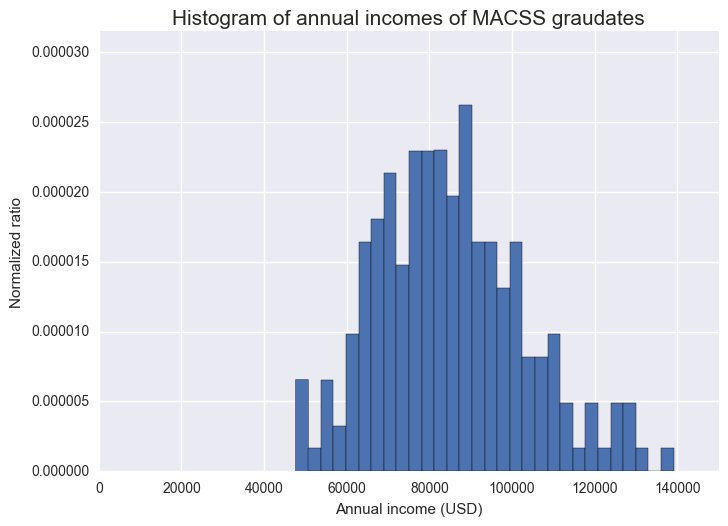
\includegraphics{./images/fig_1a.png}}}
\end{figure}
\par\bigskip

\item Estimate the parameters of the lognormal distribution by generalized method of moments. Plot your estimated lognormal PDF against the histogram from part (a). Report the value of your GMM criterion function at the estimated parameter values. Report and compare your two data moments against your two model moments at the estimated parameter values.
\par
\begin{figure}[H]\centering\captionsetup{width=4.0in}
  \fbox{\resizebox{4.0in}{3.0in}{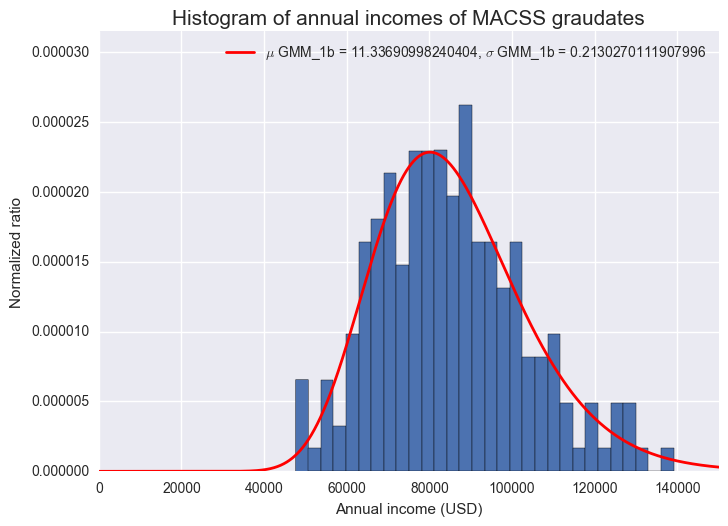
\includegraphics{./images/fig_1b.png}}}
\end{figure}
\par
GMM crietron function value = 3.93982160e-13\par
GMM estimate for $\mu$ = 11.3369099824 \par
GMM estimate for $\sigma$ = 0.213027011191\par
Data moments:\par
\hspace{2mm}Mean = 85276.8236063\par
\hspace{2mm}Standard Deviation = 17992.542128\par
Model moments:\par
\hspace{2mm}Mean = 85276.79520510265\par
\hspace{2mm}Standard Deviation = 17992.5325554\par
\bigskip

\item Perform the two-step GMM estimator by using your estimates from part (b) with two moments to generate an estimator for the variance covariance matrix. Report your estimates as well as the criterion function value at these estimates. Plot your estimated lognormal PDF against the histogram from part (a) and the estimated PDF from part (b). Report and compare your two data moments against your two model moments at the estimated parameter values.
\par\bigskip
\begin{figure}[H]\centering\captionsetup{width=4.0in}
  \fbox{\resizebox{4.0in}{3.0in}{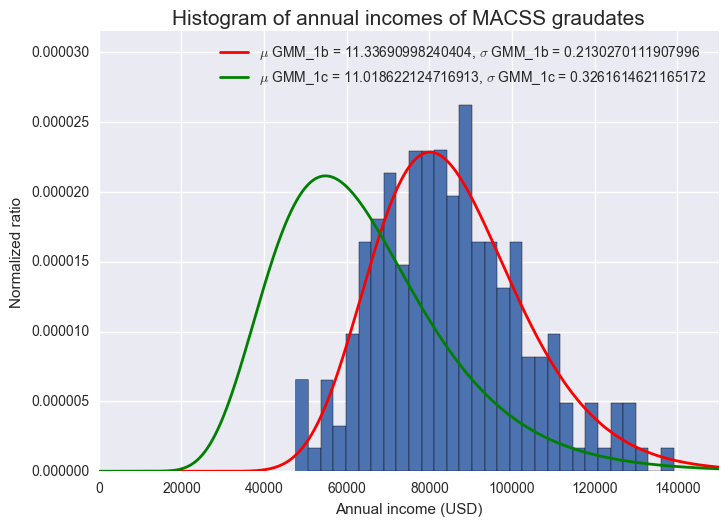
\includegraphics{./images/fig_1c.png}}}
\end{figure}
\par
GMM crietron function value = 0.08985203\par
GMM estimate for $\mu$ = 11.0186221247 \par
GMM estimate for $\sigma$ = 0.326161462117\par
Data moments:\par
\hspace{2mm} Mean = 85276.8236063\par
\hspace{2mm} Standard Deviation = 17992.542128\par
Model moments:\par
\hspace{2mm}Mean = 63849.689103934565 \par
\hspace{2mm}Standard Deviation = 20822.5632426\par
\bigskip

\item Estimate the lognormal PDF to t the data by GMM using different moments. Plot your estimated lognormal PDF against the histogram from part (a). Report the value of your GMM criterion function at the estimated parameter values. Report and compare your three data moments against your three model moments at the estimated parameter values.
\par
\begin{figure}[H]\centering\captionsetup{width=4.0in}
  \fbox{\resizebox{4.0in}{3.0in}{
\includegraphics{./images/fig_1d.png}}}
\end{figure}
\par
GMM crietron function value = 0.23818173\par
GMM estimate for $\mu$ = 11.3367266466 \par
GMM estimate for $\sigma$ = 0.211746420387\par
Data moments:\par
\hspace{2mm}\% of inidivudals who earn less than \$75,000 = 0.3\par
\hspace{2mm}\% of inidivudals who earn between \$75,000 and \$100,000 = 0.5\par
\hspace{2mm}\% of inidivudals who earn more than \$100,000 = 0.2\par
Model moments: \par
\hspace{2mm}\% of inidivudals who earn less than \$75,000 = 0.299272453678561 \par
\hspace{2mm}\% of inidivudals who earn between \$75,000 and \$100,000 = 0.4980574551520791 \par
\hspace{2mm}\% of inidivudals who earn more than \$100,000 = 0.19966278330544504
\par\bigskip

\item Perform the two-step GMM estimator by using your estimates from part (d) with three moments to generate an estimator for the variance covariance matrix. Report your estimates as well as the criterion function value at these estimates. Plot your estimated lognormal PDF against the histogram from part (a) and the estimated PDF from part (d). Report and compare your three data moments against your three model moments at the estimated parameter values.
\par\bigskip
\begin{figure}[H]\centering\captionsetup{width=4.0in}
  \fbox{\resizebox{4.0in}{3.0in}{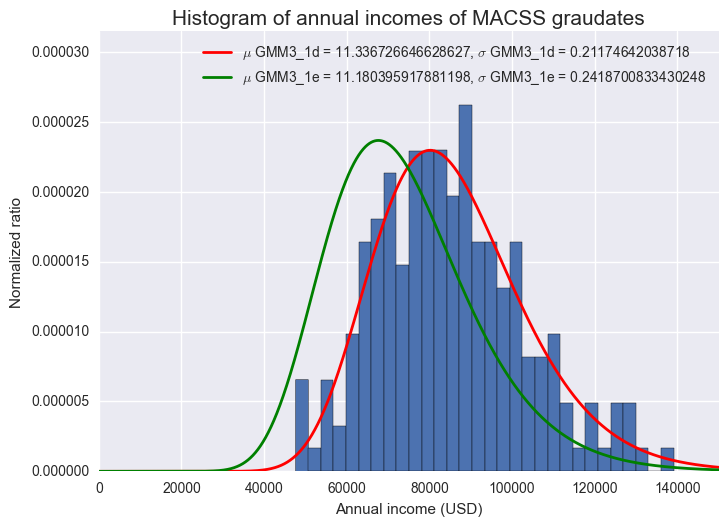
\includegraphics{./images/fig_1e.png}}}
\end{figure}
\par
GMM crietron function value = 2.89594050e-09\par
GMM estimate for $\mu$ = 11.1803959179 \par
GMM estimate for $\sigma$ = 0.241870083343\par
Data moments:\par
\hspace{2mm}\% of inidivudals who earn less than \$75,000 = 0.3\par
\hspace{2mm}\% of inidivudals who earn between \$75,000 and \$100,000 = 0.5\par
\hspace{2mm}\% of inidivudals who earn more than \$100,000 = 0.2\par
Model moments:\par
\hspace{2mm}\% of inidivudals who earn less than \$75,000 = 0.5735500650944066 \par
\hspace{2mm}\% of inidivudals who earn between \$75,000 and \$100,000 = 0.34185740892053457 \par
\hspace{2mm}\% of inidivudals who earn more than \$100,000 = 0.08345289282059601
\par\bigskip

\item Which of the four estimations from parts (b), (c), (d), and (e) ts the data best? Justify your answer.
\par\bigskip
The graphs above suggest that, for the given choice of moments and initial parameter values, the GMM estimate using the identity matrix as the weight matrix (i.e., 1.(b) and 1.(d)) fits the data better than the other using the two-step weight matrix (i.e., 1.(c) and 1.(e)). It is more difficult to compare across estimates using different moments, e.g. between 1.(b) and 1.(d). Between 1.(b) and 1.(d), the former has a slightly thinker tail than the latter, captureing more of the middle part of the histogram. It is my view that choosing the proportions of individuals for different income groups may be suprerior to choosing mean and standard deviation as moments. This is because I expect the income distribution to be generally more fat-tailed than not.

\end{enumerate}

\item \textbf{Linear regression and GMM}
\begin {enumerate}
\item Estimate the parameters of the model $(\beta_{0}, \beta_{1}, \beta_{2}, \beta_{3})$ by GMM by solving by solving the minimization problem of the GMM criterion function. Report your estimates and report the value of your GMM criterion function.
\par\bigskip

GMM estimate for $\beta_{0}$ =  0.251644953001\par
GMM estimate for $\beta_{1}$ =  0.0129334651063\par
GMM estimate for $\beta_{2}$ =  0.40050102133\par
GMM estimate for $\beta_{3}$=  -0.00999170755539\par
GMM crietron function value = 0.00182128981749\par
\end {enumerate}
\end {enumerate}

\end{document}
